%\documentclass[onecolumn, 10pt]{aastex63}
%\usepackage{graphicx}%Include figure files
\newcommand{\red}[1]{{\color{red} #1}}


%\begin{document}
\section{Proper Motion metric}


% FOM from footprint
Vera Rubin Observatory, with LSST, could conduct extensive observation of the Galaxy which can lead to the discovering of new Galactic objects and phenomena. However, the extent to which the Galactic plane will be observed within LSST is uncertain \question{refer here to the other paper?}. In addition to transients and variable, the survey may discover objects with unusual proper motion within our Galaxy, or peculiar kynematic structures, such as streams. We consider both cases in this section. 
To measure LSST's potential to discover new objects with peculiar motion, we use two approaches: we generate synthetic objects in a Monte Carlo simulation within a proper motion distribution unlike that of any known Galactic component, and we take an exemplary Galactic structure, Sagittarius A and make it fainter, and move it farther away to test the limits of different \opsim s. 

\subsection {Monte Carlo simulation of object with unusual kynematics}
We use a Monte Carlo simulation to estimate \new{LSST's ability to distinguish unusual proper motion distributions for}
 stars in different part of the sky, considering the kinematics features of the known stellar Galactic components, the bulge, 
the disk, and the stellar halo, as described in \citet{Binney2008}. 
Stars in the Galaxy have a characteristic color, luminosity, and proper motion \new{which relates to their position and probability of belonging to one of the known Galactic structures}. From the color, luminosity, and coordinates, the expected proper motion can be estimated. 

Our simulation generates the distribution of proper motion for an object of a given magnitude changing the distance, and we iterated the algorithm for all the magnitudes in the range $[15,28]$ mag in $g$ band. 

The algorithm proceeds as follows:

\begin{itemize}
    \item generation of a set of distances $\mathbf{d}$ for stars within a distance range $[0,120]$~kpc, according to the distance distribution in \citet{Binney2008};
    \item \question{MISSING assignment of each star to a galactic component according to the relative density of objects given the  distance; \question{MISSING the step where you assign the luminosity tho do you consider the magnitude in this assignment?}}
    \item random association of a position in the sky to each object we simulate according the Maxwell-Boltzmann distribution for a star in  bulge, in the disk or in the halo; \question{MISSING the step where you assign the luminosity tho do you consider the magnitude in this assignment?}
    \item draw from the velocity distribution of the component the velocity of the object (see \autoref{MB_par});
    \item from the velocity components we calculate the tangential velocity, which represents the projection of the velocity vector on the sky plane;
    \item we calculate the simulated value of the proper motion as:
    \begin{equation}\label{PM_eq}
        \mu=\frac{v_{tan}}{d~4.74}  \arcsec/yr;
    \end{equation}
\end{itemize}



The velocity distribution of the \emph{known}-objects is parametrized according to a Maxwell-Boltzmann distribution (\autoref{MB_par}), while for the \emph{unusual}-objects we propose uniform velocity distribution in the range $\left[-5000,5000\right]$ $km/s$ to mimic a different group of stars that are moving in the same dynamic structure. \question{While this is not a non-parametric model, the uniform distribution is minimally informative (is it true???)}. 

\sout{Iterating the procedure over the number of objects we want to fill the survey with, we are able to build a distribution for the \emph{usual} and \emph{unusual} objects and comparing the two} \new{not really what you do: you create distributions, not objects one by one}


From the simulation we estimate the proper motion through  \autoref{PM_eq}, \new{we calculate the observed} distance as $d=10^{(0.20*M_r+1)}$, and measure the time gap between two consecutive observations of the field \question{in the same filter? only in g right - and why consecutive observations?}. 

With this we can estimate the proper motion $\mu$, and check if it can be measured by the survey: we assume that the proper motion has to be greater of the $5\%$ of the point-spread-function (PSF) full width half maximum (FWHM) to detect the motion. \new{In order to do this we leverage a series of MAF functions: we use the time gaps metric described in \autoref{sec:timegaps}, we extract the PSF from the \opsim~ catalog, as well as the signal-to-noise ratio $\frac{S}{N}$ of the measurement of a given star, obtained from the magnitude limit for the observation which is reported in the \opsim.}



\begin{table}
\centering
\caption{\label{MB_par}The table shows the values of the parameters for the three dimensional Maxwell-Boltzmann distribution. Considering the the Galactic coordinate system, the velocity spread in the table represents a three component vector which element are its radial, transverse and axial component respectively. The form of the distribution consider also the effect from the asymmetric drift, $v_a$. $n_0$ is the normalization factor.}
\begin{tabular}{|c|c|c|c|}\hline
$f_{DF}=\frac{n_0}{(2\pi \sigma_v^2)^{3/2}}exp[-\frac{(v-v_a)^2}{\sigma_v^2}]$& $n_0$ &$v_a$[km/s] &$\sigma_v $[km/s]  \\\hline \hline
 Bulge & $0.02$ &100 & [120,95,75]  \\ \hline
 Disk & $0.98$ &10 & [40,30,20] \\ \hline
 Halo & $0.05$ &200 & [130,105,85]\\ \hline
\end{tabular}
\end{table}

The simulation let us analyse how the distribution of objects \question{SHOULD BE MORE CLEAR from a different physical background} will be observed with a given observing strategy. To understand which strategy will perform better in detecting unusual objects we measure what  fraction of unusual objects are in fact classified as unusual. To classify the object as known or unusual we use the Likelihood ratio and measure the likelihood of an object with a given set of observables  $\theta$ to belongs to the known distribution with parameters $\theta_0$ or to an unknown distribution:

\sout{which tracks the gradient of the likelihood function respect a given parameter vector }\question{dont know what tracks the gradient mean:}

\begin{equation}
    S\equiv Log\left(\frac{\mathcal{L}(\theta)}{\mathcal{L}(\theta_0)}\right),
\end{equation}
where $\mathcal{L}$ is the likelihood function, $\theta$ is the parameter vector of the object and $\theta_0$ is the parameter array for a normal distributed object in the proper motion space.

The Likelihood function is described as follow:
\begin{equation}
    \mathcal{L}\left(\mu_i|\mathbf{X}, mag, \Delta t\right)=\frac{\phi_c(\mathbf{X}_i)}{\phi(\mathbf{X}_i)} f_{DF}\left(\mathbf{v}\right)P\left(\mu|mag, \Delta t\right),
\end{equation}
where the first term of the product is the membership probability of the object to the disk, the bulge or the halo of the Galaxy, $f_{DF}\left(\mathbf{v}\right)$  is the velocity probability distribution, $P\left(\mu|mag, \Delta t\right)$ is the probability to see an object moving in a given time interval with a magnitude over the detectability threshold for a proper motion distribution.
As it had been highlighted in \citet{Kuijken02} the uncertainties on the position due to the magnitude of a moving star can be estimated as: $\sigma_{\Delta x}= \frac{S}{N}*0.67* FWHM$; since the uncertainties on the time is negligible,  $\sigma_{\Delta x}$ is the main contribution on the measurement errors, thus the probability $P\left(\mu|mag, \Delta t\right)$ can be derived as:
\begin{equation}
    P\left(\mu|mag, \Delta t\right) \approx e^{-\frac{(0.05*FWHM-\Delta t *\mu)^2 }{(0.67*FWHM)^2}*(\frac{S}{N})^2},
\end{equation}
where the term $0.05*FWHM$ is the space gap threshold for a motion to be detected, $\mu$ is the simulated proper motion, $\frac{S}{N}$ is the signal to noise ratio and $\Delta t$ is the survey duration.

\begin{figure}
\centering
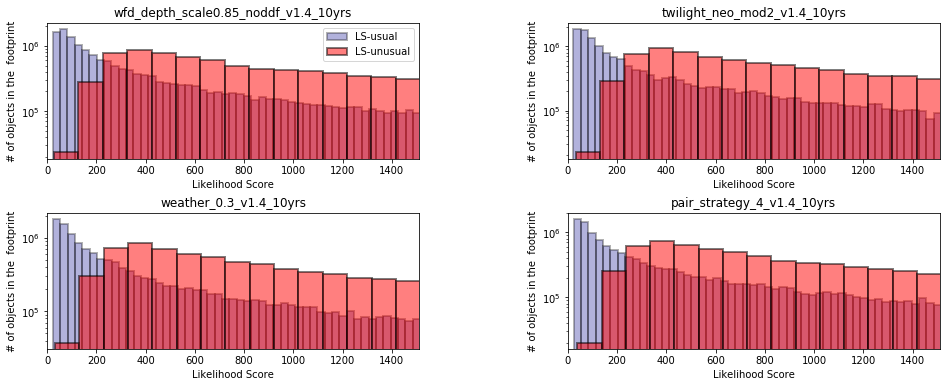
\includegraphics[scale=0.55]{figures/LS_distribution.png}
\caption{The Likelihood score distribution of simulated known and kynematically unusual objects as observed by four different \opsim s.  \question{FED: not sure what the next sentence means }. The trend of unusual object grows as the number of usual detected objects decrease. \sout{The area of the not overlapping region is related to the fraction of unusual objects detectable within the specific observation strategy, thus it is a good tracer of the \opsim~ skills.} \new{The figure of merit we define is the area of the histogram of unusual objects that is does not intersect the histogram of known objects (appropriately normalized). }}
\label{fig:PM_distribution}
\end{figure}
The Likelihood $\mathcal{L}\left(\mu_i|\mathbf{X}, mag, \Delta t\right)$, \sout{with the underlined contribution},  was used in the likelihood score estimation to track the known and unusual objects distributions, thus giving an hint on how good  a specific observation strategy is at detecting unusual observations.

\begin{figure}
\centering
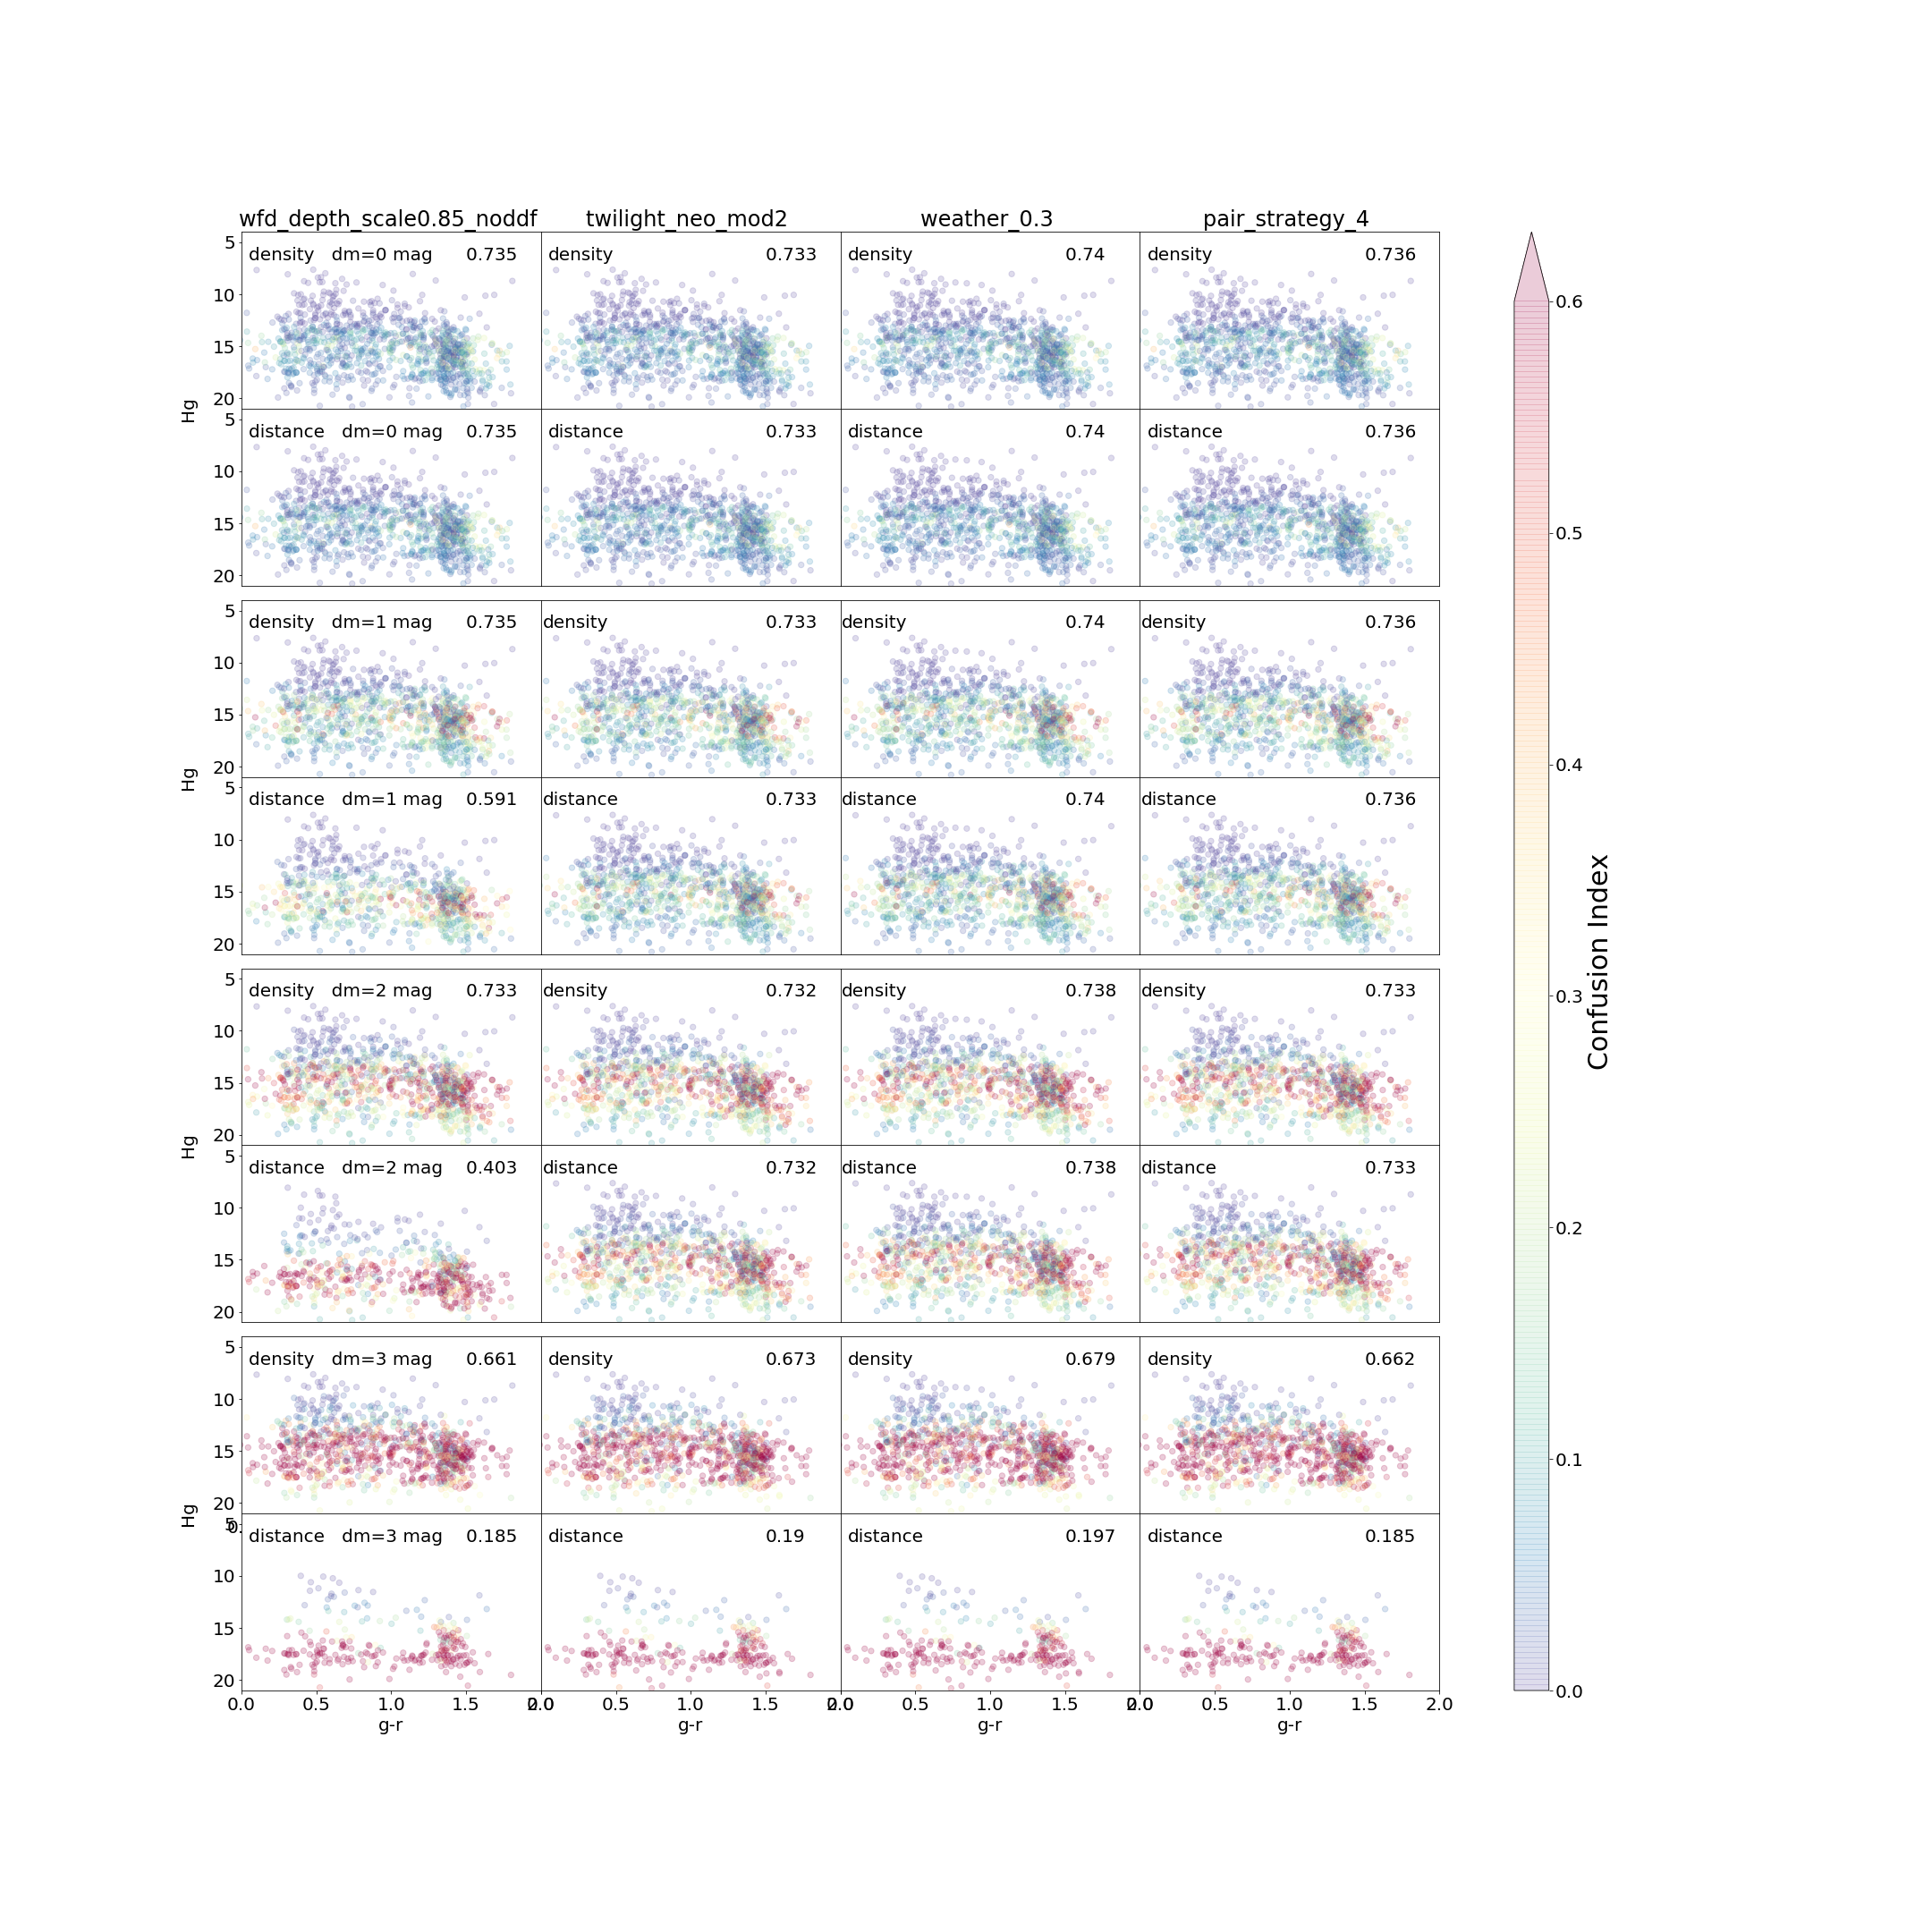
\includegraphics[scale=0.28]{figures/ConfunsionIndex_10yrs.png}
%\vspace{-20mm}
\caption{The figure presents the outcomes of the analysis on the 10 yrs survey for four different Opsims, and it shows the ability on reproducing the Proper Motion Diagram (PMD) in \citet{Carlin12} considering two possibilities: changing distance or density of Sgr. From the top to the bottom of the figure we have increased the magnitude to simulate either more distant or denser stellar structures then Sgr, the specific mode of the simulation is expressed in the top left of the plots. When we simulated changing in distance we considered related changes for the PM, following $\mu_{new}=\frac{\mu_{old}}{10^{\frac{\Delta m}{5}}}$. Looking at the top right in the plots there is shown the fraction of detected stars; we noted that  changing the distance of about $\Delta m= 3$, we already lose more than $50\%$ of the precision in detecting the proper motion and we are able to detect just about the $20\%$ of the stars in the sample. \question{remove y labels from all but the first column, put space between every 2 rows (sets of density and distance)}}
\label{fig:Conf_Idx}
\end{figure}

\subsection{Sagitarius A simulations}

\sout{ To verify the ability to support these expectations, w}

We used the Sagitarius A structure as toy model to analyze the ability of an \opsim~ to discover streams. In order to give a description on the performance of the different strategies, we reproduced the analysis from \citealt{Carlin12} on the proper motion of the \question{Sagitarius (Sgr) trail tidal debris} \sout{, using the same data set used in the cited paper (see Fig. \ref{fig:Conf_Idx}), to analyze how the science is improved in using one strategy respect another,} and we as two questions: if the stream were fainter could we still detect it? and could we detect it were farther away? To answer these questions we (1) decrease the magnitude of all stars in the dataset used in \citet{Carlin12} figure 10. This can be interpreted as probing if the same stream could be detected using main sequence stars, instead of stars in the Giant branch. (2) decrease the magnitude \emph{and the proper motion} of all stars in the dataset used in \citealt{Carlin12}, which corresponds to move the stream farther away. We measure:

\begin{itemize}
    \item the fraction of detection we lose as they exceed the magnitude limit of the survey.
    \item the fraction of stars that cannot be detected without being confused with nearby stars, \ie~ detections that fall into an error ellipse: \emph{confusion index};
    
\end{itemize}

\sout{The toy model reproduced the same structure as Sgr in two different cases:  w} We moved Sgr A  within a distance range $[28,111]$ kpc , changing the proper motion of the sources accordingly to $\mu_{new}=\frac{\mu_{old}}{10^{\frac{\Delta m}{5}}}$; we dimmed it with the range $[0,3]$ mag, changing the density of Main Sequence stars, thus letting the structure get fainter \question{when you move it away do you move it away by the correct amount that corresponds to a magnitude drop of 0, 1, 2, 3?}. 

For all \opsim s, we note that, with reference to  \autoref{fig:Conf_Idx}, we rapidly reach the $50\%$ limit in the confusion index \question{need to explain this confusion index better}. This means that for structures dimmer than Sgr A by $2$ mag we \sout{would have less sensibility in measuring colors and proper motion} only be able to use 50\% of the stars in the stream. The analysis pointed out also that for a Sgr A-like structure farther away by $111$ kpc we will be able to detect only   $\sim20\%$ of the stellar objects. 
\question{But what is the metric??}


Another important aspect we stress is the ability of the different strategies in detecting objects that moves and for which it is possible to detect the motion itself. To do that we simulated light curves that go on and off during the survey duration such as the transients can be observed at least twice, and its motion can be detected as well. \question{need more on this}


\subsection{Figure of merit}
The metrics described are able to determine, from the astrometric point of view, the best strategy to detect the proper motion. Combining them with the footprint coverage we are able to underline if there are region of the Sky that are not visited too much or not visited at all, producing a bad performance rate of the observation strategy. 
The figure of merit for a survey is defined as:
\begin{equation}
    FOM = N\frac{\sum_i MAF_i\cdot w_i}{\sum_i w_i}
\end{equation}
where $N$ is a normalization factor and the $MAF_i$ is the outcome of the metric for the \emph{i}-th field, $w_i$ is a weighted factor. The weight used is the frequency of the MAF value overall the footprint.   


\begin{figure}
    \centering
    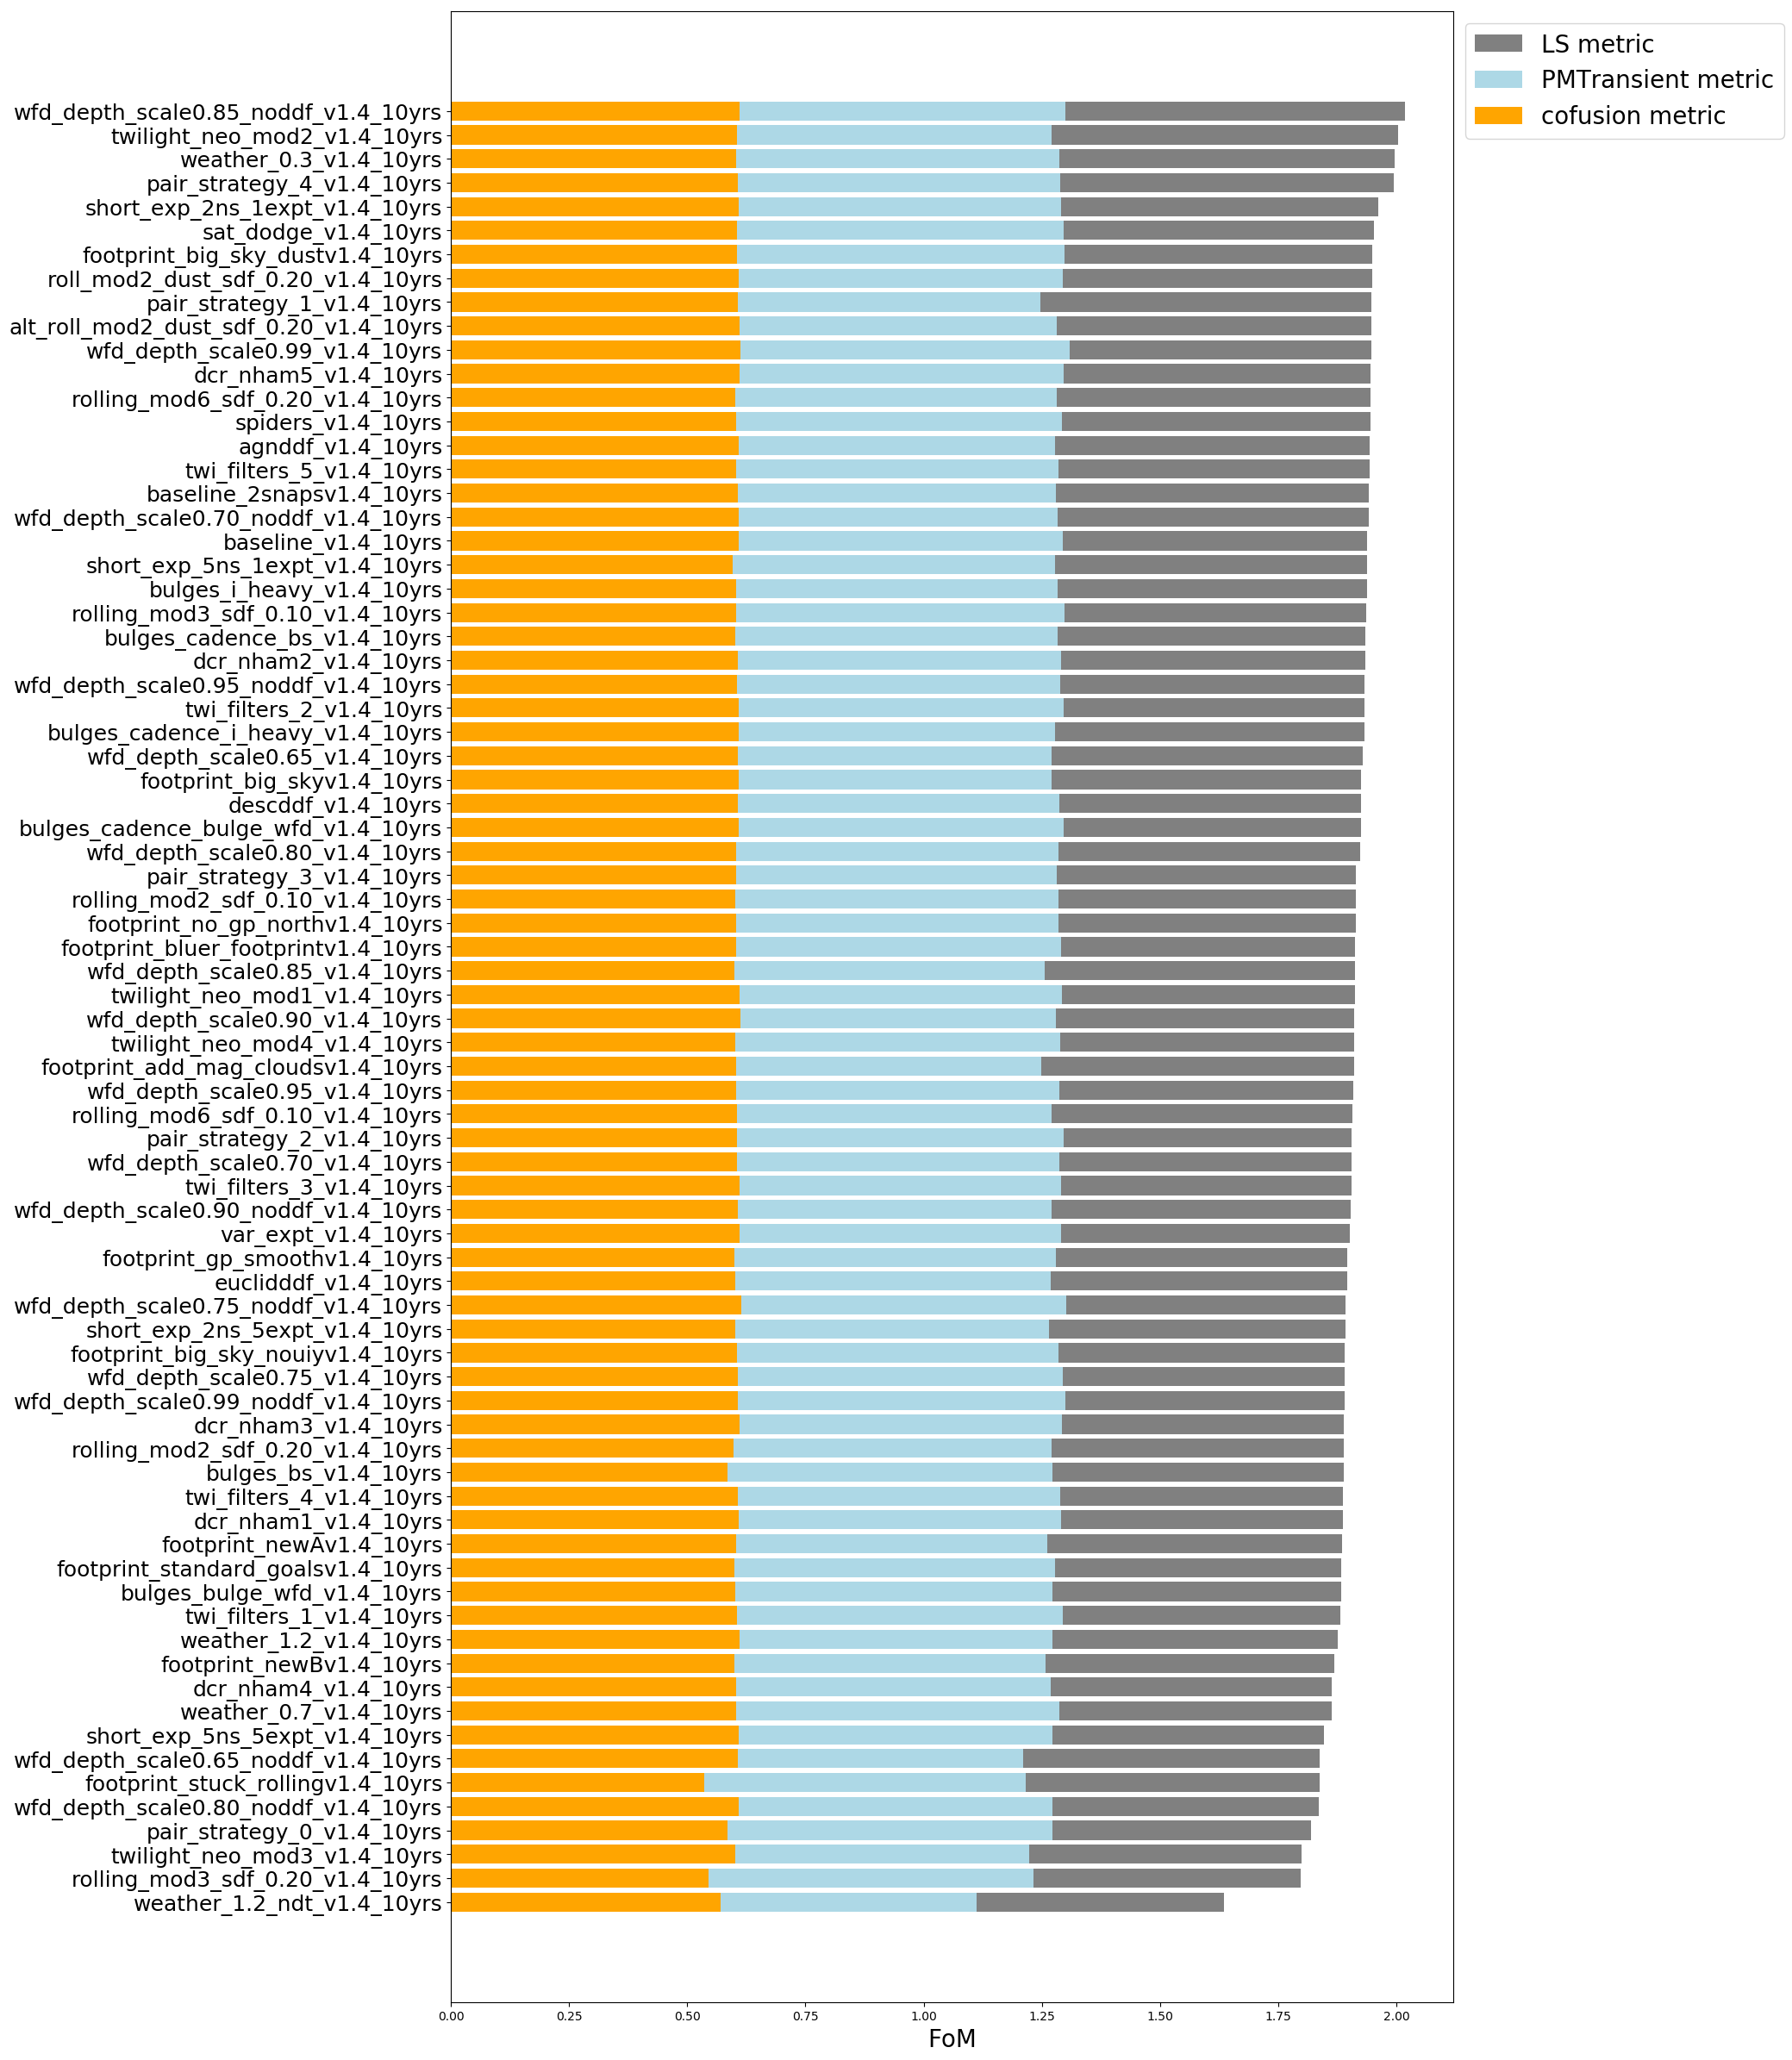
\includegraphics[scale=0.28]{figures/FOM_astrometry.png}
    \caption{}
    \label{fig:FOM_astrometry}
\end{figure}

\subsection{Results}

% \end{document}